\documentclass[lesson_slides]{subfiles}
%\usepackage{natbib}
\usepackage{graphicx}
% \graphicspath{ {./images/} }
\usepackage{enumerate}
\usepackage{pifont} % for ding
\usepackage{float} % keeps tables in the exact position they occupy in the code
\usepackage{xcolor} % text colour
\usepackage{gb4e} % leave last

\begin{document}
%%=-=-=-=-=-=-=-=-=-=-=-=-=-=-=-=-=-=-=-=-=-=-=-=-=-=-=-=-=-=-=-=-=-=-=-=-=-=-=-=
%   FRAME START   -=-=-=-=-=-=-=-=-=-=-=-=-=-=-=-=-=-=-=-=-=-=-=-=-=-=-=-=-=-=-=
\begin{frame}[c]{Overview of the data}

\textbf{\textsc{our raw data}}

\begin{table}[H]
    \centering
    \small
    \begin{adjustbox}
        \begin{tabular}{r|r|r}
        % \hline
        ESLO 1  & ESLO 2 & total \\
        \hline
        2376 & 1261 & 3637 \\
        %\hline
        \hline
        \end{tabular}
    \end{adjustbox}
\caption{\label{tab:samp3}Raw data (ex situ and in situ combined).}
\end{table}
  
\end{frame}
%   FRAME END   --==-=-=-=-=-=-=-=-=-=-=-=-=-=-=-=-=-=-=-=-=-=-=-=-=-=-=-=-=-=-=
%   FRAME START   -=-=-=-=-=-=-=-=-=-=-=-=-=-=-=-=-=-=-=-=-=-=-=-=-=-=-=-=-=-=-=
\begin{frame}[c]{Overview of the data}

\textbf{\textsc{our raw data}}

\begin{table}[H]
    \centering
    \small
    \begin{adjustbox}
        \begin{tabular}{l|rr|rr|rr|rr|rr}
        % \hline
        {} & \multicolumn{2}{c}{comment}  & \multicolumn{2}{c}{où} & \multicolumn{2}{c}{quand} & \multicolumn{2}{c}{quiO}& \multicolumn{2}{c}{quoiO}\\
        \hline
        {} & EX & IN & EX & IN & EX & IN & EX & IN & EX & IN\\
        %\hline
        1970s (eslo 1) & 848 & 37 & 233 & 72 & 156 & 38 & 42 & 13 & 333 & 198\\
        %\hline
        2010s (eslo 2) & 333 & 156 & 84 & 260 & 32 & 30 & 8 & 21 & 24 & 476 \\
        \hline
        \end{tabular}
    \end{adjustbox}
\caption{\label{tab:samp3}Total occurrences of non lexically-restricted wh-elements.}
\end{table}
  
\end{frame}
%   FRAME END   --==-=-=-=-=-=-=-=-=-=-=-=-=-=-=-=-=-=-=-=-=-=-=-=-=-=-=-=-=-=-=
%   FRAME START   -=-=-=-=-=-=-=-=-=-=-=-=-=-=-=-=-=-=-=-=-=-=-=-=-=-=-=-=-=-=-=
\begin{frame}[c]{Overview of the data}

\textbf{\textsc{our raw data}}

\begin{table}[H]
    \centering
    \small
    \begin{adjustbox}
        \begin{tabular}{l|rr|rr|rr|rr|rr}
        % \hline
        {} & \multicolumn{2}{c}{comment}  & \multicolumn{2}{c}{où} & \multicolumn{2}{c}{quand} & \multicolumn{2}{c}{quiO}& \multicolumn{2}{c}{quoiO}\\
        \hline
        {} & EX & IN & EX & IN & EX & IN & EX & IN & EX & IN\\
        %\hline
        1970s (eslo 1) & 848 & 37 & 233 & 72 & 156 & \hl{38} & 42 & 13 & 333 & 198\\
        %\hline
        2010s (eslo 2) & 333 & 156 & 84 & 260 & 32 & \hl{30} & 8 & 21 & 24 & 476 \\
        \hline
        \end{tabular}
    \end{adjustbox}
\caption{\label{tab:samp3}Total occurrences of non lexically-restricted wh-elements.}
\end{table}
  
\end{frame}
%   FRAME END   --==-=-=-=-=-=-=-=-=-=-=-=-=-=-=-=-=-=-=-=-=-=-=-=-=-=-=-=-=-=-=
%   FRAME START   -=-=-=-=-=-=-=-=-=-=-=-=-=-=-=-=-=-=-=-=-=-=-=-=-=-=-=-=-=-=-=
\begin{frame}[c]{Overview of the data}

\textbf{\textsc{our raw data}}

\begin{table}[H]
    \centering
    \small
    \begin{adjustbox}
        \begin{tabular}{l|rr|rr|rr|rr|rr}
        % \hline
        {} & \multicolumn{2}{c}{comment}  & \multicolumn{2}{c}{où} & \multicolumn{2}{c}{quand} & \multicolumn{2}{c}{quiO}& \multicolumn{2}{c}{quoiO}\\
        \hline
        {} & EX & IN & EX & IN & EX & IN & EX & IN & EX & IN\\
        %\hline
        1970s (eslo 1) & 848 & 37 & 233 & 72 & 156 & \hl{38} & 42 & \hl{13} & 333 & 198\\
        %\hline
        2010s (eslo 2) & 333 & 156 & 84 & 260 & 32 & \hl{30} & 8 & \hl{21} & 24 & 476 \\
        \hline
        \end{tabular}
    \end{adjustbox}
\caption{\label{tab:samp3}Total occurrences of non lexically-restricted wh-elements.}
\end{table}
  
\end{frame}
%   FRAME END   --==-=-=-=-=-=-=-=-=-=-=-=-=-=-=-=-=-=-=-=-=-=-=-=-=-=-=-=-=-=-=
%   FRAME START   -=-=-=-=-=-=-=-=-=-=-=-=-=-=-=-=-=-=-=-=-=-=-=-=-=-=-=-=-=-=-=
\begin{frame}[c]{The data: wh-in situ}

    \begin{center}
       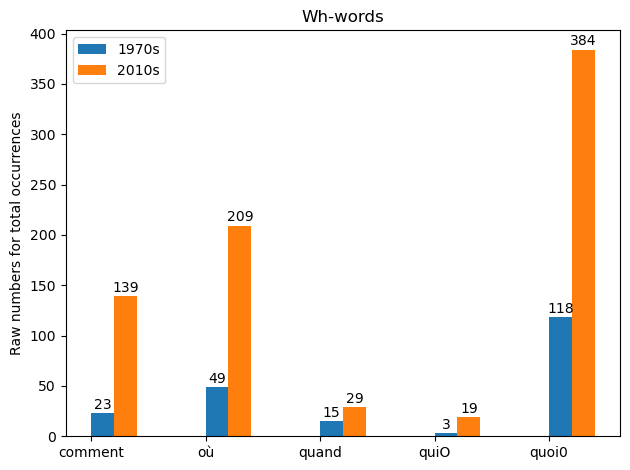
\includegraphics[width=10cm, height=6cm]{images/insituraw.png} 
    \end{center}
  
\end{frame}
%   FRAME END   --==-=-=-=-=-=-=-=-=-=-=-=-=-=-=-=-=-=-=-=-=-=-=-=-=-=-=-=-=-=-=
%   FRAME START   -=-=-=-=-=-=-=-=-=-=-=-=-=-=-=-=-=-=-=-=-=-=-=-=-=-=-=-=-=-=-=
\begin{frame}[c]{The data: wh-in situ}

    \begin{center}
       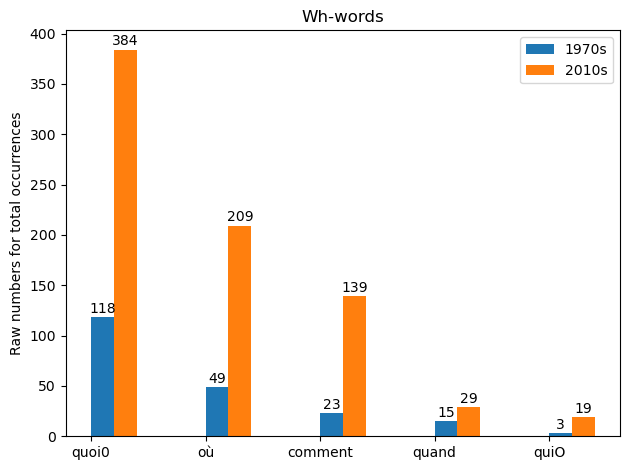
\includegraphics[width=10cm, height=6cm]{images/insituraw2.png} 
    \end{center}
  
\end{frame}
%   FRAME END   --==-=-=-=-=-=-=-=-=-=-=-=-=-=-=-=-=-=-=-=-=-=-=-=-=-=-=-=-=-=-=
%   FRAME START   -=-=-=-=-=-=-=-=-=-=-=-=-=-=-=-=-=-=-=-=-=-=-=-=-=-=-=-=-=-=-=
\begin{frame}[c]{The data: wh-in situ}

    \begin{center}
       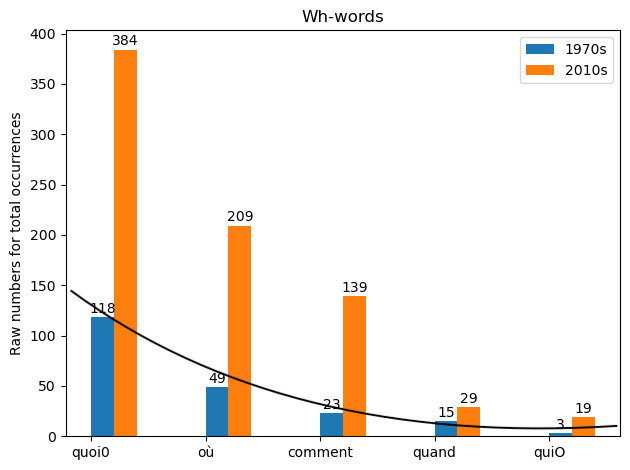
\includegraphics[width=10cm, height=6cm]{images/insituraw3.png} 
    \end{center}
  
\end{frame}
%   FRAME END   --==-=-=-=-=-=-=-=-=-=-=-=-=-=-=-=-=-=-=-=-=-=-=-=-=-=-=-=-=-=-=
%   FRAME START   -=-=-=-=-=-=-=-=-=-=-=-=-=-=-=-=-=-=-=-=-=-=-=-=-=-=-=-=-=-=-=
\begin{frame}[c]{The data: wh-in situ}

    \begin{center}
       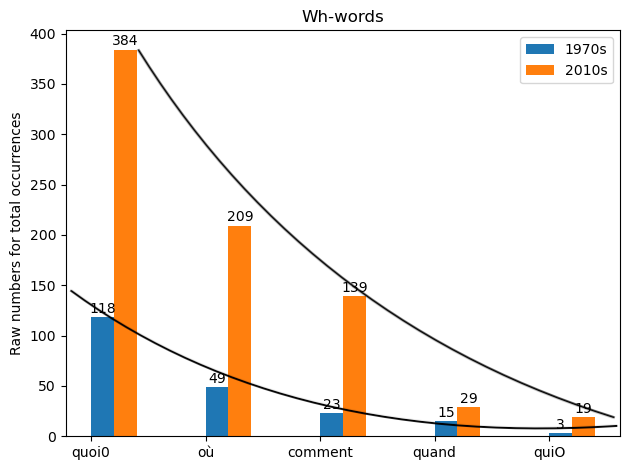
\includegraphics[width=10cm, height=6cm]{images/insituraw4.png} 
    \end{center}
  
\end{frame}
%   FRAME END   --==-=-=-=-=-=-=-=-=-=-=-=-=-=-=-=-=-=-=-=-=-=-=-=-=-=-=-=-=-=-=

%   FRAME START   -=-=-=-=-=-=-=-=-=-=-=-=-=-=-=-=-=-=-=-=-=-=-=-=-=-=-=-=-=-=-=
\begin{frame}[c]{The data: wh-in situ}

    \begin{center}
       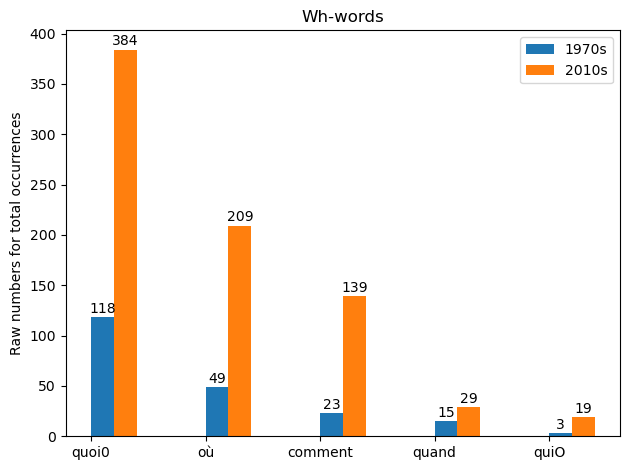
\includegraphics[width=10cm, height=6cm]{images/insituraw2.png} 
    \end{center}
  
\end{frame}
%   FRAME END   --==-=-=-=-=-=-=-=-=-=-=-=-=-=-=-=-=-=-=-=-=-=-=-=-=-=-=-=-=-=-=

%   FRAME START   -=-=-=-=-=-=-=-=-=-=-=-=-=-=-=-=-=-=-=-=-=-=-=-=-=-=-=-=-=-=-=
\begin{frame}{The classification}

    \transboxin<1>
    \transglitter<2>
    \transwipe<3>
    \textbf{\textsc{our classification}} \pause
    \begin{itemize}
        \item[\ding{227}] the \% of in situ questions > 1 (Larrivée's threshold for categorial values)\\ \pause $\longrightarrow$ we expected wh-in situ to \textbf{not} be categorical \pause (not just explicitly-activated) \pause
        \item[\ding{227}] we determined three activation levels (using both the script and the audio file): \pause
        \item[\ding{227}] explicitly activated ($=$ prepositional content repeated in the question) \pause
        \item[\ding{227}] non-activated ($=$ 'discourse new') \pause
        \item[\ding{227}] \textbf{inferable} \pause (Garassino 2021)
            
    \end{itemize}

\end{frame}
%   FRAME END   --==-=-=-=-=-=-=-=-=-=-=-=-=-=-=-=-=-=-=-=-=-=-=-=-=-=-=-=-=-=-=
%   FRAME START   -=-=-=-=-=-=-=-=-=-=-=-=-=-=-=-=-=-=-=-=-=-=-=-=-=-=-=-=-=-=-=
\begin{frame}{The classification}

    \textbf{\textsc{our classification}}
    \begin{itemize}
        \item[\ding{227}] the \% of in situ questions > 1 (Larrivée's threshold for categorial values)\\ $\longrightarrow$ we expected wh-in situ to \textbf{not} be categorical (not just explicitly-activated)
        \item[\ding{227}] we determined three activation levels (using both the script and the audio file):
        \item[\ding{227}] explicitly activated ($=$ prepositional content repeated in the question)
        \item[\ding{227}] \underline{non-activated} ($=$ 'discourse new')
        \item[\ding{227}] \textbf{inferable} (Garassino 2021)
            
    \end{itemize}

\end{frame}
%   FRAME END   --==-=-=-=-=-=-=-=-=-=-=-=-=-=-=-=-=-=-=-=-=-=-=-=-=-=-=-=-=-=-=
%   FRAME START   -=-=-=-=-=-=-=-=-=-=-=-=-=-=-=-=-=-=-=-=-=-=-=-=-=-=-=-=-=-=-=
\begin{frame}{The classification}

    \textbf{\textsc{our classification}}
    \begin{itemize}
        \item[\ding{227}] the \% of in situ questions > 1 (Larrivée's threshold for categorial values)\\ $\longrightarrow$ we expected wh-in situ to \textbf{not} be categorical (not just explicitly-activated)
        \item[\ding{227}] we determined three activation levels (using both the script and the audio file):
        \item[\ding{227}] explicitly activated ($=$ prepositional content repeated in the question)
        \item[\ding{227}] \underline{non-activated} ($=$ '\textcolor{red}{discourse new}')
        \item[\ding{227}] \textbf{inferable} (Garassino 2021)
            
    \end{itemize}

\end{frame}
%   FRAME END   --==-=-=-=-=-=-=-=-=-=-=-=-=-=-=-=-=-=-=-=-=-=-=-=-=-=-=-=-=-=-=
%   FRAME START   -=-=-=-=-=-=-=-=-=-=-=-=-=-=-=-=-=-=-=-=-=-=-=-=-=-=-=-=-=-=-=
\begin{frame}{The classification}

    \textbf{\textsc{our classification}}
    \begin{itemize}
        \item[\ding{227}] the \% of in situ questions > 1 (Larrivée's threshold for categorial values)\\ $\longrightarrow$ we expected wh-in situ to \textbf{not} be categorical (not just explicitly-activated)
        \item[\ding{227}] we determined three activation levels (using both the script and the audio file):
        \item[\ding{227}] explicitly activated ($=$ prepositional content repeated in the question) $=$ '\textcolor{blue}{discourse old}'
        \item[\ding{227}] \underline{non-activated} ($=$ '\textcolor{red}{discourse new}')
        \item[\ding{227}] \textbf{inferable} (Garassino 2021)
            
    \end{itemize}

\end{frame}
%   FRAME END   --==-=-=-=-=-=-=-=-=-=-=-=-=-=-=-=-=-=-=-=-=-=-=-=-=-=-=-=-=-=-=
%   FRAME START   -=-=-=-=-=-=-=-=-=-=-=-=-=-=-=-=-=-=-=-=-=-=-=-=-=-=-=-=-=-=-=
\begin{frame}{The classification}

    \textbf{\textsc{our classification}}
    \begin{itemize}
        \item[\ding{227}] the \% of in situ questions > 1 (Larrivée's threshold for categorial values)\\ $\longrightarrow$ we expected wh-in situ to \textbf{not} be categorical (not just explicitly-activated)
        \item[\ding{227}] we determined three activation levels (using both the script and the audio file):
        \item[\ding{227}] explicitly activated ($=$ prepositional content repeated in the question) $=$ '\textcolor{blue}{discourse old}'
        \item[\ding{227}] \underline{non-activated} ($=$ '\textcolor{red}{discourse new}')
        \item[\ding{227}] \textbf{inferable} (Garassino 2021) $=$ '\textcolor{blue}{discourse old}'
            
    \end{itemize}

\end{frame}
%   FRAME END   --==-=-=-=-=-=-=-=-=-=-=-=-=-=-=-=-=-=-=-=-=-=-=-=-=-=-=-=-=-=-=
%   FRAME START   -=-=-=-=-=-=-=-=-=-=-=-=-=-=-=-=-=-=-=-=-=-=-=-=-=-=-=-=-=-=-=
\begin{frame}{The classification}

    \transboxin<1>
    \transglitter<2>
    \transwipe<3>
    \textbf{\textsc{inferable wh-in situ}}\\ \pause
    The propositional content of the question is not “explicitly mentioned in the conversation, but is easily accessible thanks to our world knowledge’ (Garassino 2021: 10). \pause 

    \begin{exe}
        \ex C-ORAL-ROM, ffamcv05 (Garassino 2021 : 10, (12))
 \pause
        \begin{xlist}
            \exi{NAT:} Et qu’est-ce que tu as acheté d’autre alors ? \pause
            \exi{MAI:} Et ben on a acheté...euh la table avec les quatre chaises...sept-cent balles... \pause
            \exi{JOS:} Pour mettre \textbf{où} ?
        \end{xlist} 
    \end{exe}

\end{frame}
%   FRAME END   --==-=-=-=-=-=-=-=-=-=-=-=-=-=-=-=-=-=-=-=-=-=-=-=-=-=-=-=-=-=-=
%   FRAME START   -=-=-=-=-=-=-=-=-=-=-=-=-=-=-=-=-=-=-=-=-=-=-=-=-=-=-=-=-=-=-=
\begin{frame}{The classification}

    \transboxin<1>
    \transglitter<2>
    \transwipe<3>
    \textbf{\textsc{research questions}} \pause 
    \begin{itemize}
        \item[\ding{227}] Q1:  \pause To what extent does the overall proportion between in-situ and ex-situ vary over time? \pause
        \item[\ding{227}] Q2: \pause To what extent does the proportion of explicitly activated / inferable / non-activated vary over time? \pause
        \item[\ding{227}] Q3: \pause To what extent does the proportion of Discourse Old (explicitly activated $+$ inferable) vs Discourse New (non activated) vary over time?
    \end{itemize}

\end{frame}
%   FRAME END   --==-=-=-=-=-=-=-=-=-=-=-=-=-=-=-=-=-=-=-=-=-=-=-=-=-=-=-=-=-=-=
%   FRAME START   -=-=-=-=-=-=-=-=-=-=-=-=-=-=-=-=-=-=-=-=-=-=-=-=-=-=-=-=-=-=-=
\begin{frame}[c]{French wh-interrogatives from 1870 to 2014}

    \begin{center}
        \textbf{To what extent does the overall proportion between in-situ and ex-situ vary over time?}
    \end{center}
  
\end{frame}
%   FRAME END   --==-=-=-=-=-=-=-=-=-=-=-=-=-=-=-=-=-=-=-=-=-=-=-=-=-=-=-=-=-=-=
%   FRAME START   -=-=-=-=-=-=-=-=-=-=-=-=-=-=-=-=-=-=-=-=-=-=-=-=-=-=-=-=-=-=-=
\begin{frame}[c]{From predominant wh-ex situ to predominant wh-in situ}

    \transboxin<1>
    \transglitter<2>
    %\transwipe<3>
    \textbf{\textsc{the decline of wh-ex situ}} \pause (all types combined) \pause
    \begin{center}
        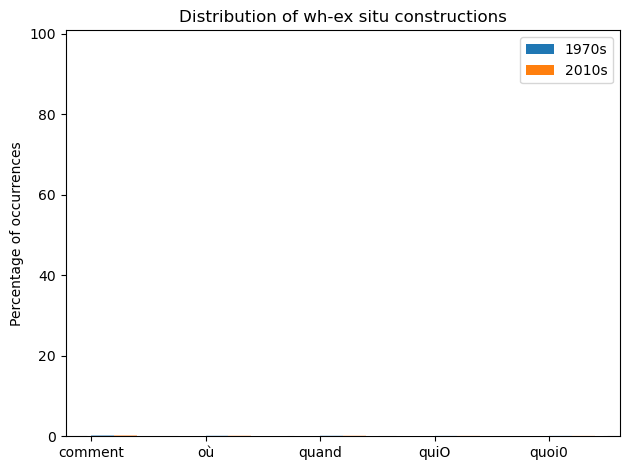
\includegraphics[width=10cm, height=6cm]{images/exsituempty.png}
    \end{center}
  
\end{frame}
%   FRAME END   --==-=-=-=-=-=-=-=-=-=-=-=-=-=-=-=-=-=-=-=-=-=-=-=-=-=-=-=-=-=-=
%   FRAME START   -=-=-=-=-=-=-=-=-=-=-=-=-=-=-=-=-=-=-=-=-=-=-=-=-=-=-=-=-=-=-=
\begin{frame}[c]{From predominant wh-ex situ to predominant wh-in situ}

    \textbf{\textsc{the decline of wh-ex situ}} (all types combined)
    \begin{center}
        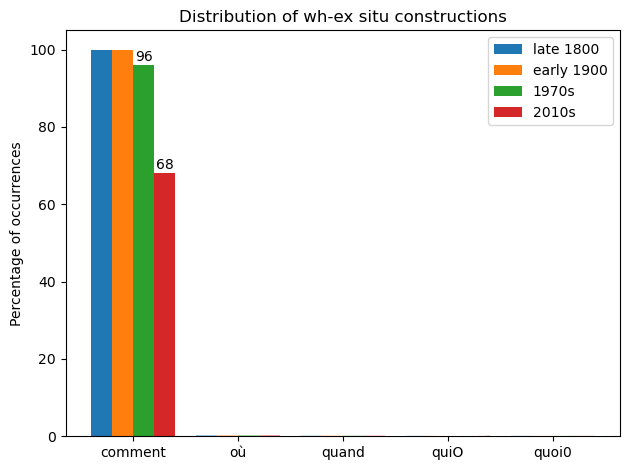
\includegraphics[width=10cm, height=6cm]{images/exsitu1.png}
    \end{center}
  
\end{frame}
%   FRAME END   --==-=-=-=-=-=-=-=-=-=-=-=-=-=-=-=-=-=-=-=-=-=-=-=-=-=-=-=-=-=-=
%   FRAME START   -=-=-=-=-=-=-=-=-=-=-=-=-=-=-=-=-=-=-=-=-=-=-=-=-=-=-=-=-=-=-=
\begin{frame}[c]{From predominant wh-ex situ to predominant wh-in situ}

    \textbf{\textsc{the decline of wh-ex situ}} (all types combined)
    \begin{center}
        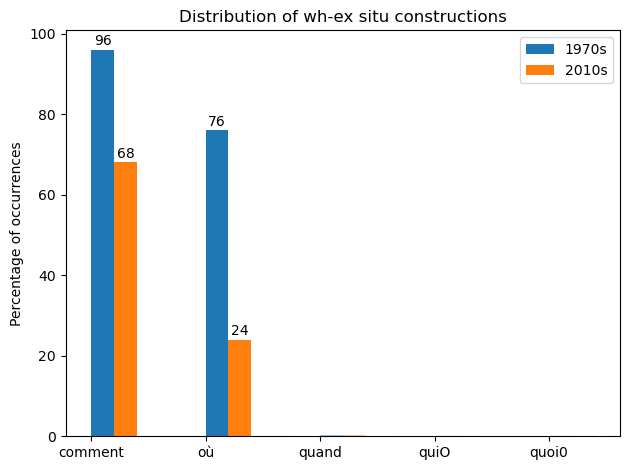
\includegraphics[width=10cm, height=6cm]{images/exsitu2.png}
    \end{center}
  
\end{frame}
%   FRAME END   --==-=-=-=-=-=-=-=-=-=-=-=-=-=-=-=-=-=-=-=-=-=-=-=-=-=-=-=-=-=-=
%   FRAME START   -=-=-=-=-=-=-=-=-=-=-=-=-=-=-=-=-=-=-=-=-=-=-=-=-=-=-=-=-=-=-=
\begin{frame}[c]{From predominant wh-ex situ to predominant wh-in situ}

    \textbf{\textsc{the decline of wh-ex situ}} (all types combined)
    \begin{center}
        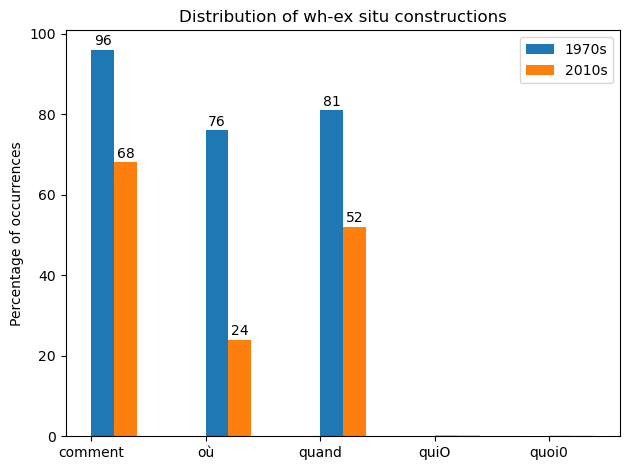
\includegraphics[width=10cm, height=6cm]{images/exsitu3.png}
    \end{center}
  
\end{frame}
%   FRAME END   --==-=-=-=-=-=-=-=-=-=-=-=-=-=-=-=-=-=-=-=-=-=-=-=-=-=-=-=-=-=-=
%   FRAME START   -=-=-=-=-=-=-=-=-=-=-=-=-=-=-=-=-=-=-=-=-=-=-=-=-=-=-=-=-=-=-=
\begin{frame}[c]{From predominant wh-ex situ to predominant wh-in situ}

    \textbf{\textsc{the decline of wh-ex situ}} (all types combined)
    \begin{center}
        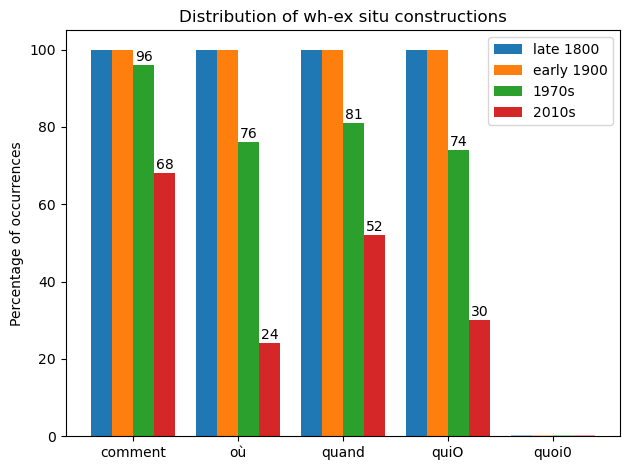
\includegraphics[width=10cm, height=6cm]{images/exsitu4.png}
    \end{center}
  
\end{frame}
%   FRAME END   --==-=-=-=-=-=-=-=-=-=-=-=-=-=-=-=-=-=-=-=-=-=-=-=-=-=-=-=-=-=-=
%   FRAME START   -=-=-=-=-=-=-=-=-=-=-=-=-=-=-=-=-=-=-=-=-=-=-=-=-=-=-=-=-=-=-=
\begin{frame}[c]{From predominant wh-ex situ to predominant wh-in situ}

    \textbf{\textsc{the decline of wh-ex situ}} (all types combined)
    \begin{center}
        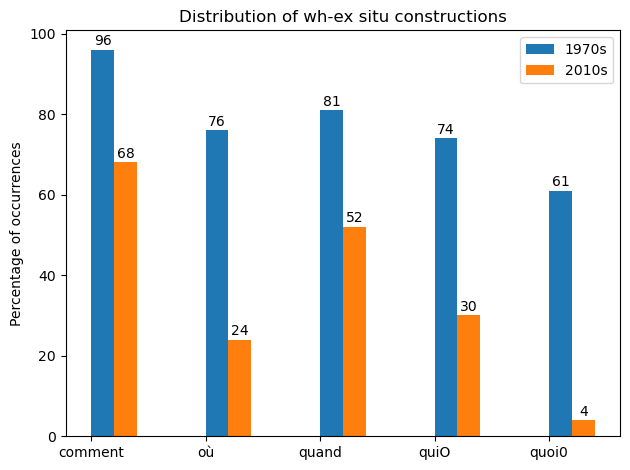
\includegraphics[width=10cm, height=6cm]{images/exsituall.png}
    \end{center}
  
\end{frame}
%   FRAME END   --==-=-=-=-=-=-=-=-=-=-=-=-=-=-=-=-=-=-=-=-=-=-=-=-=-=-=-=-=-=-=
%   FRAME START   -=-=-=-=-=-=-=-=-=-=-=-=-=-=-=-=-=-=-=-=-=-=-=-=-=-=-=-=-=-=-=
\begin{frame}[c]{From predominant wh-ex situ to predominant wh-in situ}

    \transboxin<1>
    \transglitter<2>
    %\transwipe<3>
    \textbf{\textsc{the rise of wh-in situ}} \pause
    \begin{center}
        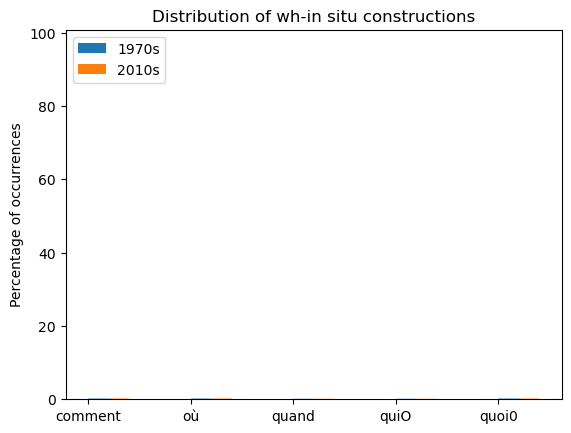
\includegraphics[width=10cm, height=6cm]{images/insituempty.png}
    \end{center}
  
\end{frame}
%   FRAME END   --==-=-=-=-=-=-=-=-=-=-=-=-=-=-=-=-=-=-=-=-=-=-=-=-=-=-=-=-=-=-=
%   FRAME START   -=-=-=-=-=-=-=-=-=-=-=-=-=-=-=-=-=-=-=-=-=-=-=-=-=-=-=-=-=-=-=
\begin{frame}[c]{From predominant wh-ex situ to predominant wh-in situ}


    \textbf{\textsc{the rise of wh-in situ}}
    \begin{center}
        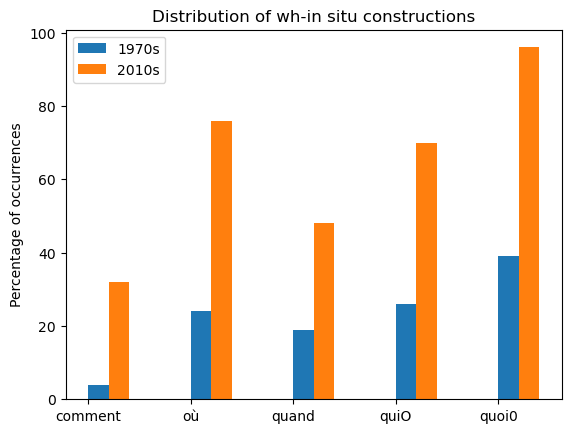
\includegraphics[width=10cm, height=6cm]{images/insitub.png}
    \end{center}
  
\end{frame}
%   FRAME END   --==-=-=-=-=-=-=-=-=-=-=-=-=-=-=-=-=-=-=-=-=-=-=-=-=-=-=-=-=-=-=
%   FRAME START   -=-=-=-=-=-=-=-=-=-=-=-=-=-=-=-=-=-=-=-=-=-=-=-=-=-=-=-=-=-=-=
\begin{frame}[c]{From predominant wh-ex situ to predominant wh-in situ}

    \transboxin<1>
    \transglitter<2>
    %\transwipe<3>
    \textbf{\textsc{general overview}} \pause
    \begin{center}
        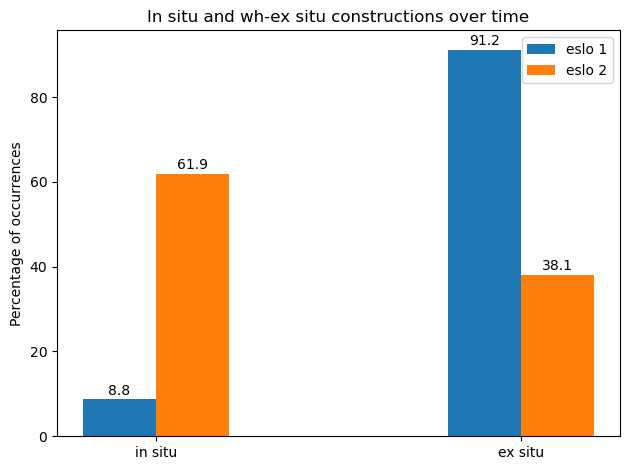
\includegraphics[width=10cm, height=6cm]{images/exsituinsituperc.png}
    \end{center}
  
\end{frame}
%   FRAME END   --==-=-=-=-=-=-=-=-=-=-=-=-=-=-=-=-=-=-=-=-=-=-=-=-=-=-=-=-=-=-=
%   FRAME START   -=-=-=-=-=-=-=-=-=-=-=-=-=-=-=-=-=-=-=-=-=-=-=-=-=-=-=-=-=-=-=
\begin{frame}[c]{From predominant wh-ex situ to predominant wh-in situ}

    \textbf{\textsc{general overview}}
    \begin{center}
        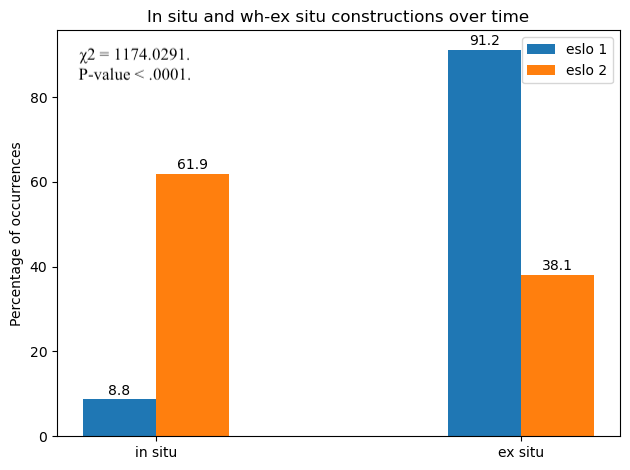
\includegraphics[width=10cm, height=6cm]{images/exsituinsituperc2.png}
    \end{center}
  
\end{frame}
%   FRAME END   --==-=-=-=-=-=-=-=-=-=-=-=-=-=-=-=-=-=-=-=-=-=-=-=-=-=-=-=-=-=-=
%   FRAME START   -=-=-=-=-=-=-=-=-=-=-=-=-=-=-=-=-=-=-=-=-=-=-=-=-=-=-=-=-=-=-=
\begin{frame}[c]{From predominant wh-ex situ to predominant wh-in situ}

    \textbf{\textsc{general overview}}
    \begin{center}
        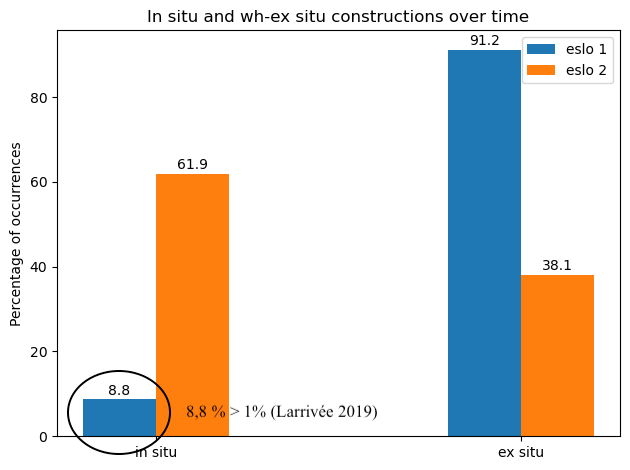
\includegraphics[width=10cm, height=6cm]{images/exsituinsituperc4.png}
    \end{center}
  
\end{frame}
%   FRAME END   --==-=-=-=-=-=-=-=-=-=-=-=-=-=-=-=-=-=-=-=-=-=-=-=-=-=-=-=-=-=-=
%   FRAME START   -=-=-=-=-=-=-=-=-=-=-=-=-=-=-=-=-=-=-=-=-=-=-=-=-=-=-=-=-=-=-=
\begin{frame}[c]{French wh-interrogatives from 1870 to 2014}

    \begin{center}
        \textbf{To what extent does the proportion of explicitly activated / inferable / non-activated vary over time?}
    \end{center}
  
\end{frame}
%   FRAME END   --==-=-=-=-=-=-=-=-=-=-=-=-=-=-=-=-=-=-=-=-=-=-=-=-=-=-=-=-=-=-=
%   FRAME START   -=-=-=-=-=-=-=-=-=-=-=-=-=-=-=-=-=-=-=-=-=-=-=-=-=-=-=-=-=-=-=
\begin{frame}[c]{Towards an increase of non-activation}

    \transboxin<1>
    \transglitter<2>
    %\transwipe<3>
    \textbf{\textsc{levels of activation over time}} \pause
    \begin{center}
        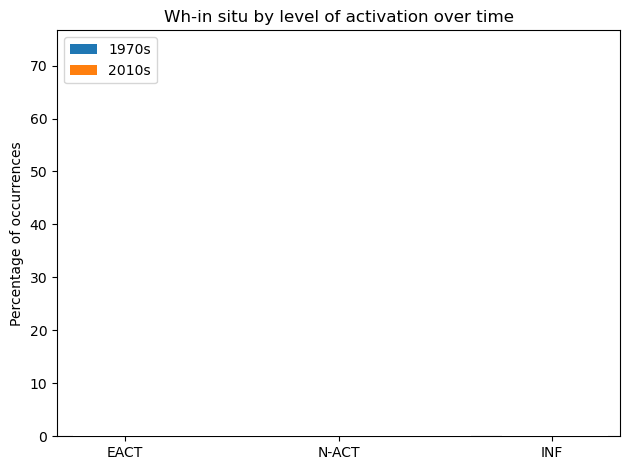
\includegraphics[width=10cm, height=6cm]{images/activationsempty.png}
    \end{center}
  
\end{frame}
%   FRAME END   --==-=-=-=-=-=-=-=-=-=-=-=-=-=-=-=-=-=-=-=-=-=-=-=-=-=-=-=-=-=-=
%   FRAME START   -=-=-=-=-=-=-=-=-=-=-=-=-=-=-=-=-=-=-=-=-=-=-=-=-=-=-=-=-=-=-=
\begin{frame}[c]{Towards an increase of non-activation}

    \textbf{\textsc{levels of activation over time}}
    \begin{center}
        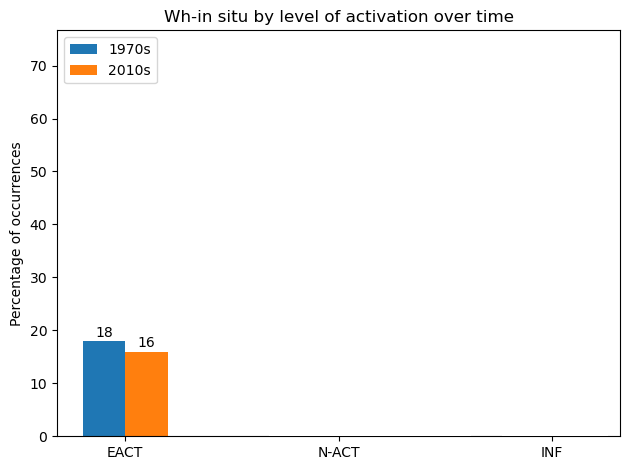
\includegraphics[width=10cm, height=6cm]{images/activations1.png}
    \end{center}
  
\end{frame}
%   FRAME END   --==-=-=-=-=-=-=-=-=-=-=-=-=-=-=-=-=-=-=-=-=-=-=-=-=-=-=-=-=-=-=
%   FRAME START   -=-=-=-=-=-=-=-=-=-=-=-=-=-=-=-=-=-=-=-=-=-=-=-=-=-=-=-=-=-=-=
\begin{frame}[c]{Towards an increase of non-activation}

    \textbf{\textsc{levels of activation over time}}
    \begin{center}
        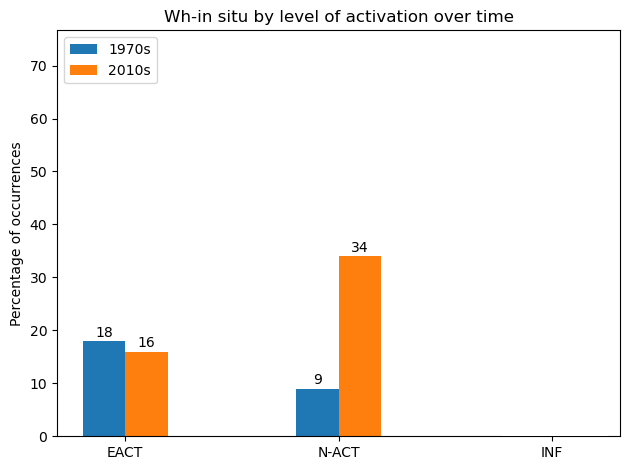
\includegraphics[width=10cm, height=6cm]{images/activations2.png}
    \end{center}
  
\end{frame}
%   FRAME END   --==-=-=-=-=-=-=-=-=-=-=-=-=-=-=-=-=-=-=-=-=-=-=-=-=-=-=-=-=-=-=
%   FRAME START   -=-=-=-=-=-=-=-=-=-=-=-=-=-=-=-=-=-=-=-=-=-=-=-=-=-=-=-=-=-=-=
\begin{frame}[c]{Towards an increase of non-activation}

    \textbf{\textsc{levels of activation over time}}
    \begin{center}
        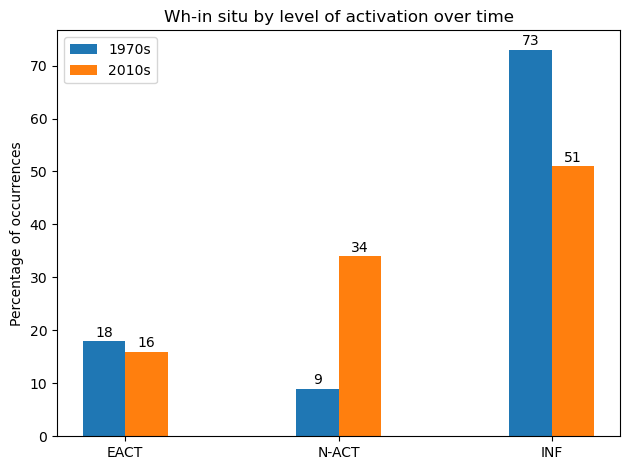
\includegraphics[width=10cm, height=6cm]{images/activationsall.png}
    \end{center}
  
\end{frame}
%   FRAME END   --==-=-=-=-=-=-=-=-=-=-=-=-=-=-=-=-=-=-=-=-=-=-=-=-=-=-=-=-=-=-=
%   FRAME START   -=-=-=-=-=-=-=-=-=-=-=-=-=-=-=-=-=-=-=-=-=-=-=-=-=-=-=-=-=-=-=
\begin{frame}[c]{Towards an increase of non-activation}

    \textbf{\textsc{levels of activation over time}}
    \begin{center}
        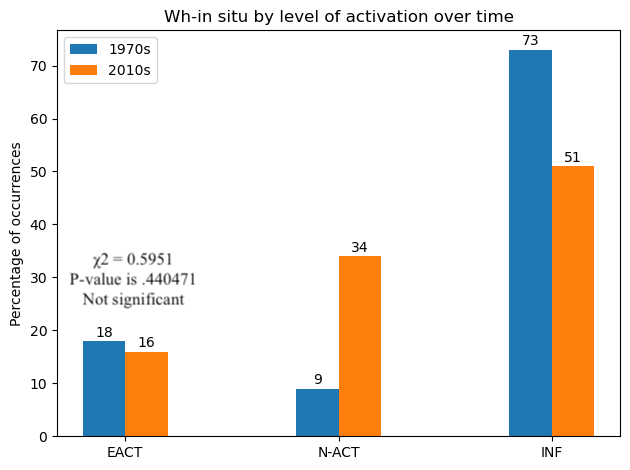
\includegraphics[width=10cm, height=6cm]{images/activationschi.png}
    \end{center}
  
\end{frame}
%   FRAME END   --==-=-=-=-=-=-=-=-=-=-=-=-=-=-=-=-=-=-=-=-=-=-=-=-=-=-=-=-=-=-=
%   FRAME START   -=-=-=-=-=-=-=-=-=-=-=-=-=-=-=-=-=-=-=-=-=-=-=-=-=-=-=-=-=-=-=
\begin{frame}[c]{Towards an increase of non-activation}

    \textbf{\textsc{levels of activation over time}}
    \begin{center}
        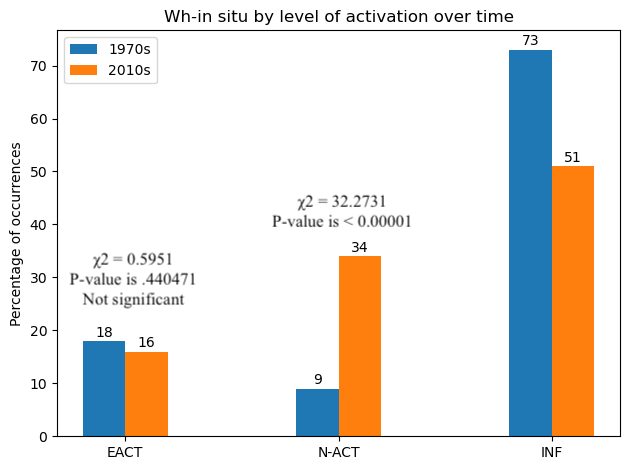
\includegraphics[width=10cm, height=6cm]{images/activationschi2.png}
    \end{center}
  
\end{frame}
%   FRAME END   --==-=-=-=-=-=-=-=-=-=-=-=-=-=-=-=-=-=-=-=-=-=-=-=-=-=-=-=-=-=-=
%   FRAME START   -=-=-=-=-=-=-=-=-=-=-=-=-=-=-=-=-=-=-=-=-=-=-=-=-=-=-=-=-=-=-=
\begin{frame}[c]{Towards an increase of non-activation}

    \textbf{\textsc{levels of activation over time}}
    \begin{center}
        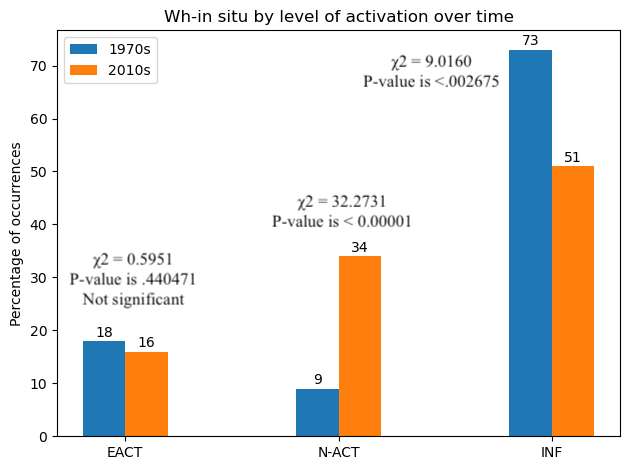
\includegraphics[width=10cm, height=6cm]{images/activationschi3.png}
    \end{center}
  
\end{frame}
%   FRAME END   --==-=-=-=-=-=-=-=-=-=-=-=-=-=-=-=-=-=-=-=-=-=-=-=-=-=-=-=-=-=-=
%   FRAME START   -=-=-=-=-=-=-=-=-=-=-=-=-=-=-=-=-=-=-=-=-=-=-=-=-=-=-=-=-=-=-=
\begin{frame}[c]{Towards an increase of non-activation}

    \textbf{\textsc{levels of activation over time}}
    \begin{center}
        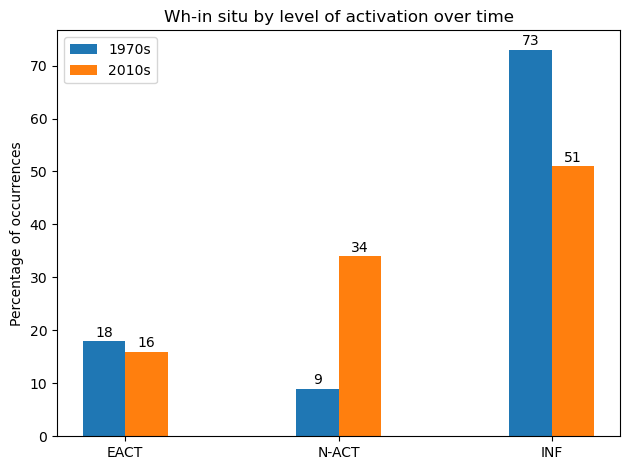
\includegraphics[width=10cm, height=6cm]{images/activationsallb.png}
    \end{center}
  
\end{frame}
%   FRAME END   --==-=-=-=-=-=-=-=-=-=-=-=-=-=-=-=-=-=-=-=-=-=-=-=-=-=-=-=-=-=-=
%   FRAME START   -=-=-=-=-=-=-=-=-=-=-=-=-=-=-=-=-=-=-=-=-=-=-=-=-=-=-=-=-=-=-=
\begin{frame}[c]{Towards an increase of non-activation}

    \textbf{\textsc{levels of activation over time}}
    \begin{center}
        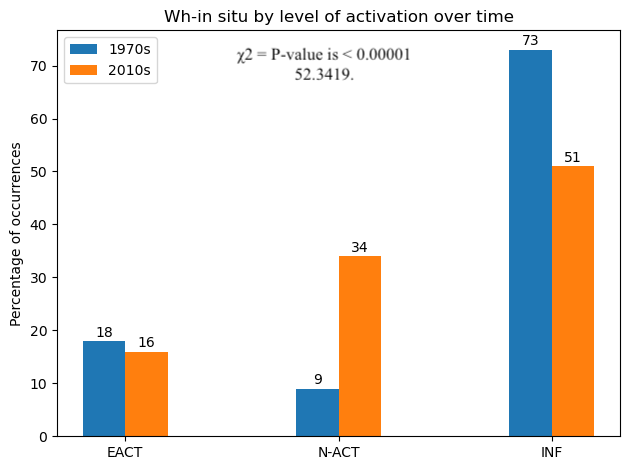
\includegraphics[width=10cm, height=6cm]{images/activationsallb2.png}
    \end{center}
  
\end{frame}
%   FRAME END   --==-=-=-=-=-=-=-=-=-=-=-=-=-=-=-=-=-=-=-=-=-=-=-=-=-=-=-=-=-=-=
%   FRAME START   -=-=-=-=-=-=-=-=-=-=-=-=-=-=-=-=-=-=-=-=-=-=-=-=-=-=-=-=-=-=-=
\begin{frame}[c]{Towards an increase of non-activation}

    \textbf{\textsc{levels of activation over time}}
    \begin{center}
        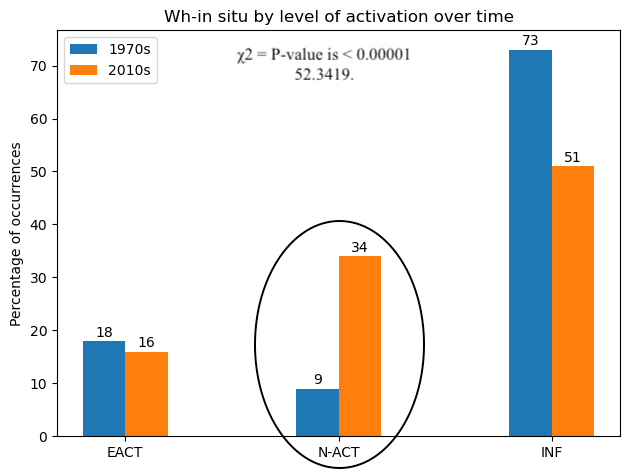
\includegraphics[width=10cm, height=6cm]{images/activationsallb3.png}
    \end{center}
  
\end{frame}
%   FRAME END   --==-=-=-=-=-=-=-=-=-=-=-=-=-=-=-=-=-=-=-=-=-=-=-=-=-=-=-=-=-=-=
%   FRAME START   -=-=-=-=-=-=-=-=-=-=-=-=-=-=-=-=-=-=-=-=-=-=-=-=-=-=-=-=-=-=-=
\begin{frame}[c]{French wh-interrogatives from 1870 to 2014}

    \begin{center}
        \textbf{To what extent does the proportion of Discourse Old vs Discourse New vary over time?}
    \end{center}
  
\end{frame}
%   FRAME END   --==-=-=-=-=-=-=-=-=-=-=-=-=-=-=-=-=-=-=-=-=-=-=-=-=-=-=-=-=-=-=
\begin{frame}[c]{Non-activation drives the change}

    \textbf{\textsc{discourse-old vs discourse new over time}}
    \begin{center}
        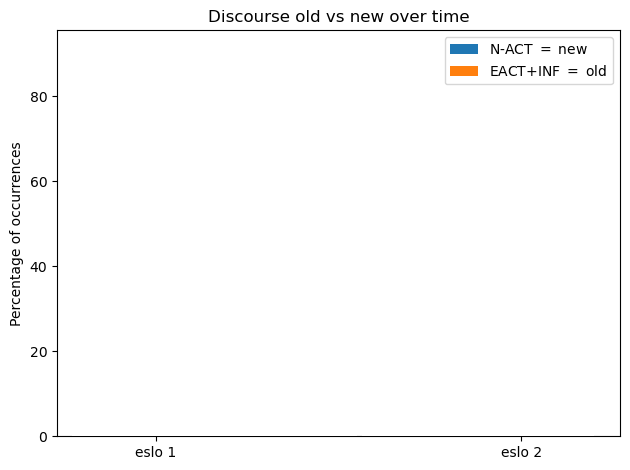
\includegraphics[width=10cm, height=6cm]{images/oldnew1empty.png}
    \end{center}
  
\end{frame}
%   FRAME END   --==-=-=-=-=-=-=-=-=-=-=-=-=-=-=-=-=-=-=-=-=-=-=-=-=-=-=-=-=-=-=
\begin{frame}[c]{Non-activation drives the change}

    \textbf{\textsc{discourse-old vs discourse new over time}}
    \begin{center}
        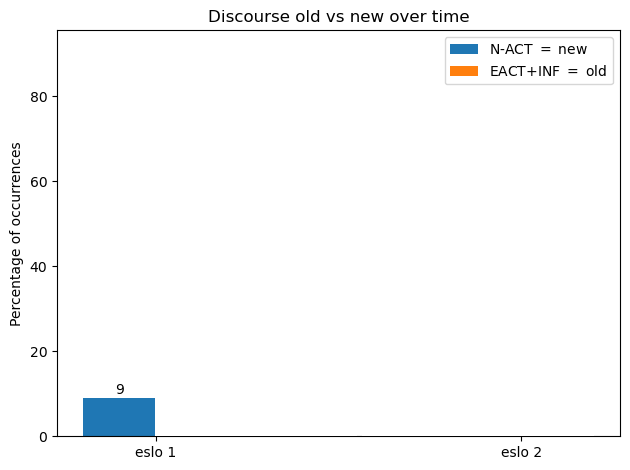
\includegraphics[width=10cm, height=6cm]{images/oldnew1.png}
    \end{center}
  
\end{frame}
%   FRAME END   --==-=-=-=-=-=-=-=-=-=-=-=-=-=-=-=-=-=-=-=-=-=-=-=-=-=-=-=-=-=-=
\begin{frame}[c]{Non-activation drives the change}

    \textbf{\textsc{discourse-old vs discourse new over time}}
    \begin{center}
        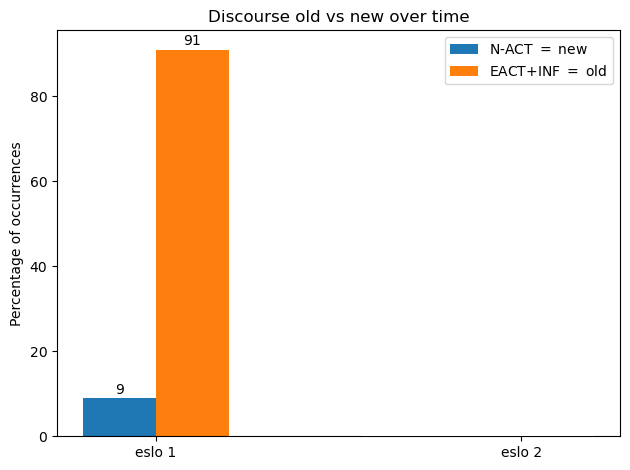
\includegraphics[width=10cm, height=6cm]{images/oldnew2.png}
    \end{center}
  
\end{frame}
%   FRAME END   --==-=-=-=-=-=-=-=-=-=-=-=-=-=-=-=-=-=-=-=-=-=-=-=-=-=-=-=-=-=-=
\begin{frame}[c]{Non-activation drives the change}

    \textbf{\textsc{discourse-old vs discourse new over time}}
    \begin{center}
        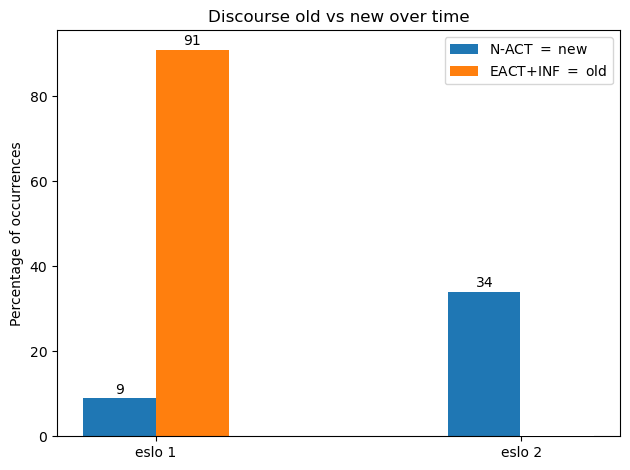
\includegraphics[width=10cm, height=6cm]{images/oldnew3.png}
    \end{center}
  
\end{frame}
%   FRAME END   --==-=-=-=-=-=-=-=-=-=-=-=-=-=-=-=-=-=-=-=-=-=-=-=-=-=-=-=-=-=-=
\begin{frame}[c]{Non-activation drives the change}

    \textbf{\textsc{discourse-old vs discourse new over time}}
    \begin{center}
        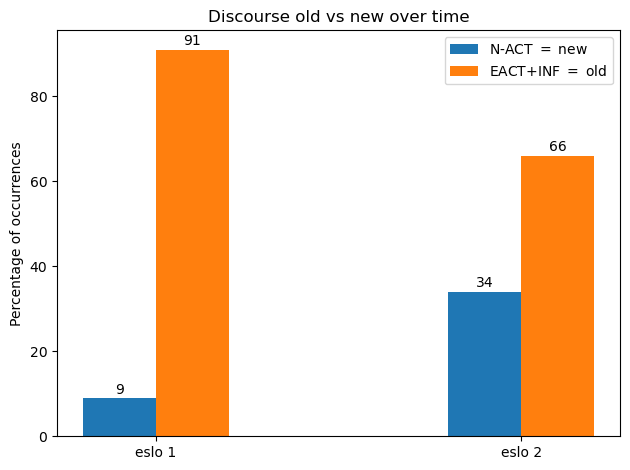
\includegraphics[width=10cm, height=6cm]{images/oldnewall.png}
    \end{center}
  
\end{frame}
%   FRAME END   --==-=-=-=-=-=-=-=-=-=-=-=-=-=-=-=-=-=-=-=-=-=-=-=-=-=-=-=-=-=-=
\begin{frame}[c]{Non-activation drives the change}

    \textbf{\textsc{discourse-old vs discourse new over time}}
    \begin{center}
        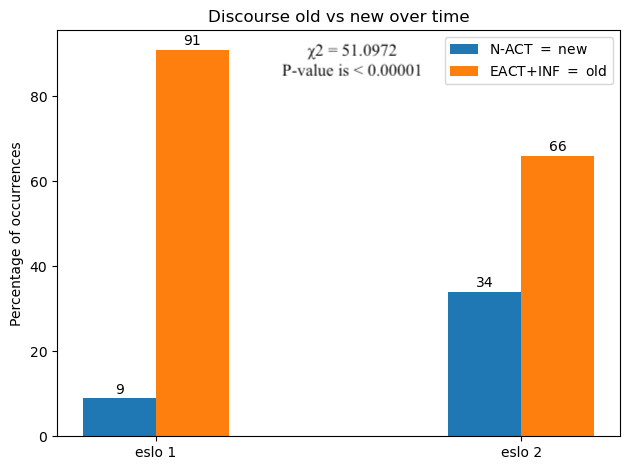
\includegraphics[width=10cm, height=6cm]{images/oldnewallchi.png}
    \end{center}
  
\end{frame}
%   FRAME END   --==-=-=-=-=-=-=-=-=-=-=-=-=-=-=-=-=-=-=-=-=-=-=-=-=-=-=-=-=-=-=
%   FRAME END   --==-=-=-=-=-=-=-=-=-=-=-=-=-=-=-=-=-=-=-=-=-=-=-=-=-=-=-=-=-=-=
\begin{frame}[c]{Summing up}

    \transboxin<1>
    \transglitter<2>
    %\transwipe<3>
    \textbf{\textsc{summary}} \pause
    \begin{center}
        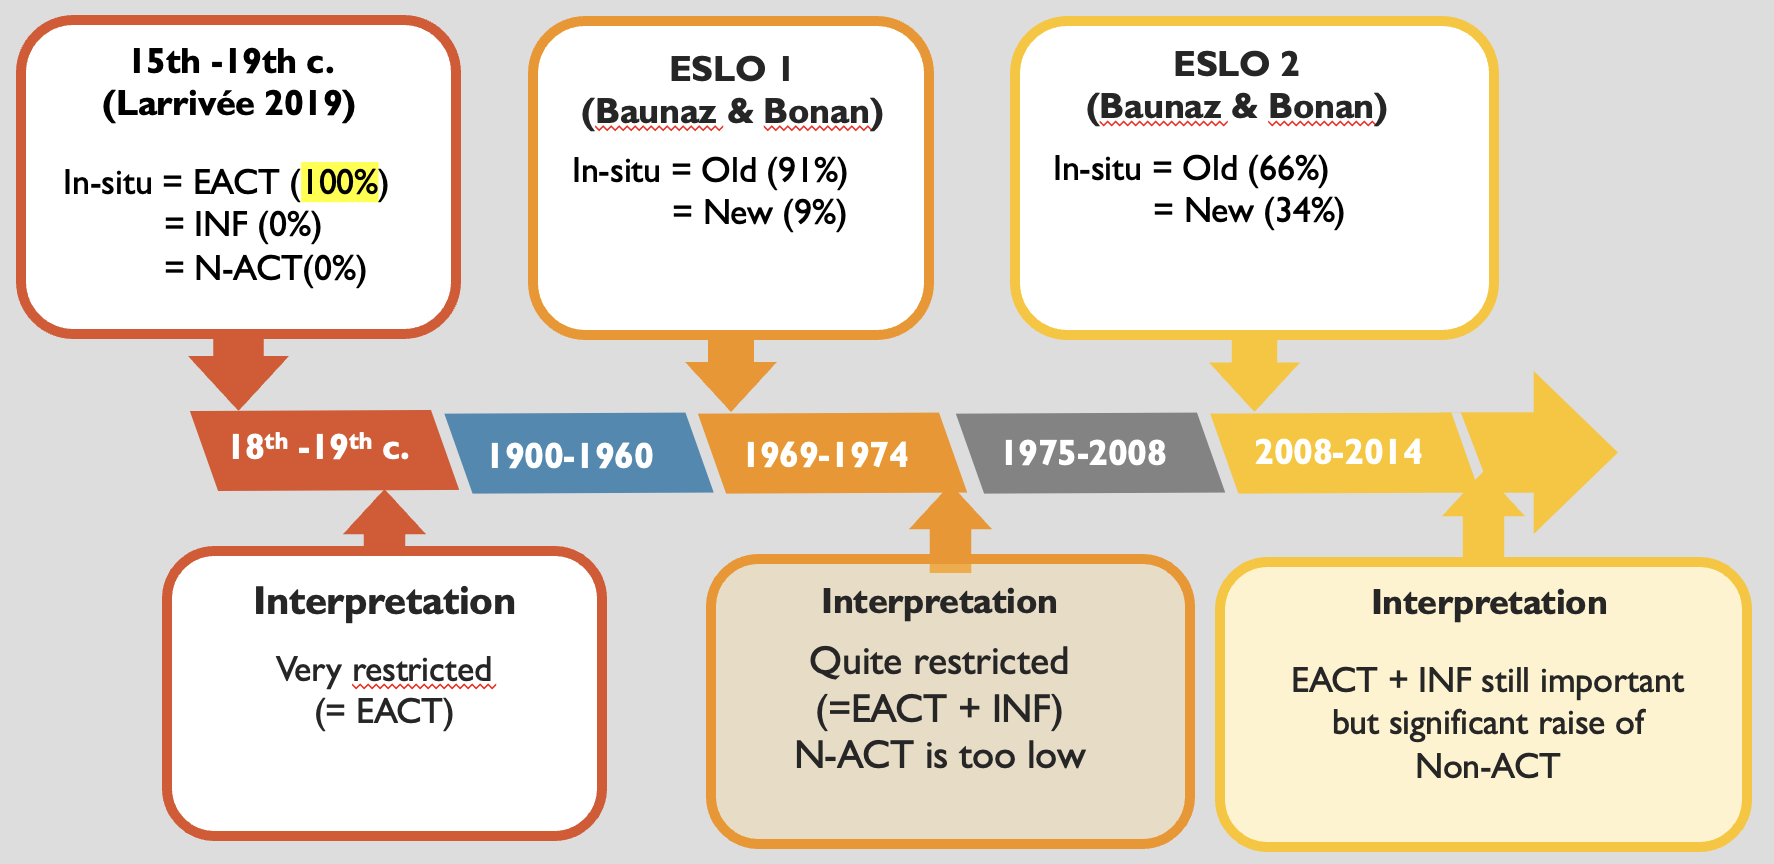
\includegraphics[width=10cm, height=6cm]{images/summary.png}
    \end{center}
  
\end{frame}
%   FRAME END   --==-=-=-=-=-=-=-=-=-=-=-=-=-=-=-=-=-=-=-=-=-=-=-=-=-=-=-=-=-=-=
%   FRAME END   --==-=-=-=-=-=-=-=-=-=-=-=-=-=-=-=-=-=-=-=-=-=-=-=-=-=-=-=-=-=-=
\begin{frame}[c]{Summing up}

    \transboxin<1>
    \transglitter<2>
    %\transwipe<3>
    \textbf{\textsc{the controversy}} \pause
    \begin{itemize}
        \item[\ding{227}] conservatives (mid 1990s - 2000s);\\ \pause
        \item[\ding{227}] liberals (mid 2000s - today)\\
    \end{itemize}
  
\end{frame}
%   FRAME END   --==-=-=-=-=-=-=-=-=-=-=-=-=-=-=-=-=-=-=-=-=-=-=-=-=-=-=-=-=-=-=
%   FRAME END   --==-=-=-=-=-=-=-=-=-=-=-=-=-=-=-=-=-=-=-=-=-=-=-=-=-=-=-=-=-=-=
\begin{frame}[c]{Summing up}

    \transboxin<1>
    \transglitter<2>
    %\transwipe<3>
    \textbf{\textsc{the controversy}}
    \begin{itemize}
        \item[\ding{227}] conservatives (mid 1990s - 2000s);\\ $\longrightarrow$ compatible with ESLO 1 data \pause (little N-ACT, mostly discourse-old wh-in situ)
        \item[\ding{227}] liberals (mid 2000s - today)\\
    \end{itemize}
  
\end{frame}
%   FRAME END   --==-=-=-=-=-=-=-=-=-=-=-=-=-=-=-=-=-=-=-=-=-=-=-=-=-=-=-=-=-=-=
%   FRAME END   --==-=-=-=-=-=-=-=-=-=-=-=-=-=-=-=-=-=-=-=-=-=-=-=-=-=-=-=-=-=-=
\begin{frame}[c]{Summing up}

    \transboxin<1>
    \transglitter<2>
    %\transwipe<3>
    \textbf{\textsc{the controversy}}
    \begin{itemize}
        \item[\ding{227}] conservatives (mid 1990s - 2000s);\\ $\longrightarrow$ compatible with ESLO 1 data (little N-ACT, mostly discourse-old wh-in situ)
        \item[\ding{227}] liberals (mid 2000s - today)\\
        $\longrightarrow$ compatible with ESLO 2 data \pause (numerous N-ACT, i.e. discourse new)
    \end{itemize}
  
\end{frame}
%   FRAME END   --==-=-=-=-=-=-=-=-=-=-=-=-=-=-=-=-=-=-=-=-=-=-=-=-=-=-=-=-=-=-=
\end{document}